% ai-assist Presentation
% Compile with: pdflatex ai-assist-presentation.tex (run twice)
\documentclass[aspectratio=169,10pt]{beamer}

\usetheme{metropolis}

% ── Red Hat Branding ──────────────────────────────────────────────
\definecolor{rhred}{HTML}{EE0000}
\definecolor{rhdarkgray}{HTML}{2D2D2D}
\definecolor{rhlightgray}{HTML}{F2F2F2}
\definecolor{rhwhite}{HTML}{FFFFFF}
\definecolor{rhblue}{HTML}{0066CC}
\definecolor{rhgreen}{HTML}{3E8635}
\definecolor{rhorange}{HTML}{EC7A08}
\definecolor{rhpurple}{HTML}{6753AC}
\definecolor{rhteal}{HTML}{009596}

\setbeamercolor{palette primary}{bg=rhdarkgray,fg=rhwhite}
\setbeamercolor{frametitle}{bg=rhred,fg=rhwhite}
\setbeamercolor{progress bar}{fg=rhred}
\setbeamercolor{alerted text}{fg=rhred}
\setbeamercolor{example text}{fg=rhgreen}
\setbeamercolor{title separator}{fg=rhred}
\setbeamercolor{progress bar in head/foot}{fg=rhred,bg=rhlightgray}
\setbeamercolor{progress bar in section page}{fg=rhred,bg=rhlightgray}

% ── Packages ──────────────────────────────────────────────────────
\usepackage{tikz}
\usetikzlibrary{shapes.geometric,arrows.meta,positioning,calc,fit,decorations.pathreplacing}
\usepackage{listings}
\usepackage{fancyvrb}
\usepackage{appendixnumberbeamer}
\usepackage{booktabs}
\usepackage{graphicx}
\usepackage{hyperref}
\usepackage[T1]{fontenc}

% ── Listings Style ────────────────────────────────────────────────
\lstdefinestyle{code}{
  basicstyle=\ttfamily\scriptsize,
  keywordstyle=\color{rhblue}\bfseries,
  stringstyle=\color{rhgreen},
  commentstyle=\color{gray}\itshape,
  backgroundcolor=\color{rhlightgray},
  frame=single,
  rulecolor=\color{gray!30},
  breaklines=true,
  showstringspaces=false,
  tabsize=2,
  xleftmargin=2mm,
  xrightmargin=2mm,
}
\lstdefinestyle{yaml}{
  style=code,
  morekeywords={servers,command,args,env,enabled,tasks,name,prompt,interval,notify},
}
\lstdefinestyle{json}{
  style=code,
  morekeywords={},
  morestring=[b]",
}
\lstdefinestyle{python}{
  style=code,
  language=Python,
  morekeywords={async,await,dataclass,Self},
}

% ── Metadata ──────────────────────────────────────────────────────
\title{ai-assist}
\subtitle{An AI-Powered Assistant for Engineering Teams}
\author{Fr\'ed\'eric Lepied\\{\small Senior Manager -- Telco Partner CI}}
\date{2026}
\institute{Red Hat}

% ══════════════════════════════════════════════════════════════════
\begin{document}

% ── Slide 1: Title ────────────────────────────────────────────────
\maketitle

% ══════════════════════════════════════════════════════════════════
\section{The Problem}
% ══════════════════════════════════════════════════════════════════

% ── Slide 2: The Problem ─────────────────────────────────────────
\begin{frame}[fragile]{The Daily Grind}
\begin{columns}[T]
\begin{column}{0.45\textwidth}
\begin{itemize}
  \item Engineers juggle DCI jobs, Jira tickets, multiple dashboards
  \item Managers need summaries but lack time for deep dives
  \item Knowledge is scattered across systems
  \item Failures repeat --- lessons are not captured
  \item Periodic manual checks are tedious and error-prone
\end{itemize}
\end{column}
\begin{column}{0.50\textwidth}
\centering
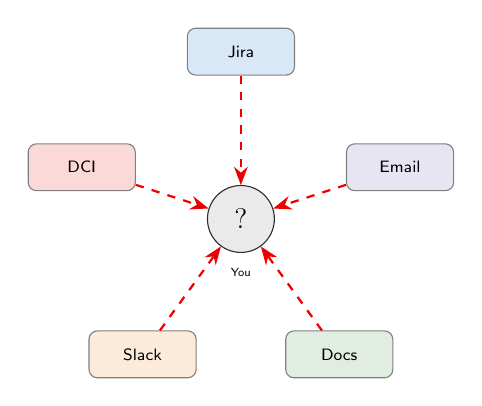
\begin{tikzpicture}[
  source/.style={rounded corners=3pt, draw=gray, fill=rhlightgray,
    font=\scriptsize\sffamily, minimum width=1.6cm, minimum height=0.7cm},
  scale=0.85, transform shape
]
  % Person in center
  \node[circle, draw=rhdarkgray, fill=rhdarkgray!10, minimum size=1cm,
    font=\large] (person) {?};
  \node[below=1mm of person, font=\tiny\sffamily] {You};

  % Data sources around the person
  \node[source, fill=rhblue!15] (jira) at (90:2.5cm) {Jira};
  \node[source, fill=rhred!15] (dci) at (162:2.5cm) {DCI};
  \node[source, fill=rhorange!15] (slack) at (234:2.5cm) {Slack};
  \node[source, fill=rhgreen!15] (docs) at (306:2.5cm) {Docs};
  \node[source, fill=rhpurple!15] (email) at (18:2.5cm) {Email};

  % Arrows
  \draw[-{Stealth}, rhred, thick, dashed] (jira) -- (person);
  \draw[-{Stealth}, rhred, thick, dashed] (dci) -- (person);
  \draw[-{Stealth}, rhred, thick, dashed] (slack) -- (person);
  \draw[-{Stealth}, rhred, thick, dashed] (docs) -- (person);
  \draw[-{Stealth}, rhred, thick, dashed] (email) -- (person);
\end{tikzpicture}
\end{column}
\end{columns}
\end{frame}

% ── Slide 3: The Vision ──────────────────────────────────────────
\begin{frame}[fragile]{What If Your AI Knew the Context?}
\begin{columns}[T]
\begin{column}{0.45\textwidth}
\begin{itemize}
  \item A single assistant that \alert{monitors} your systems 24/7
  \item \alert{Remembers} lessons, preferences, and decisions over time
  \item \alert{Connects} the dots between failures, tickets, and past learnings
  \item Generates \alert{reports} and sends \alert{notifications} automatically
  \item \alert{Extensible} via MCP servers and Agent Skills
\end{itemize}
\end{column}
\begin{column}{0.50\textwidth}
\centering
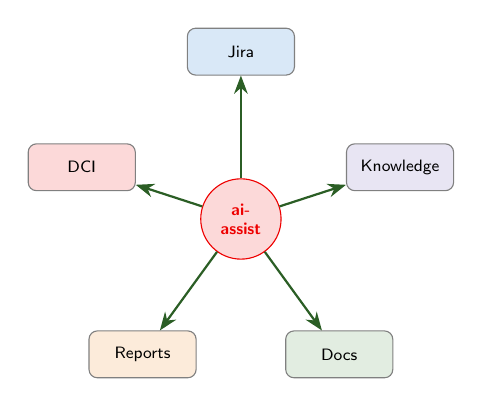
\begin{tikzpicture}[
  source/.style={rounded corners=3pt, draw=gray, fill=rhlightgray,
    font=\scriptsize\sffamily, minimum width=1.6cm, minimum height=0.7cm},
  scale=0.85, transform shape
]
  % ai-assist hub
  \node[circle, draw=rhred, fill=rhred!15, minimum size=1.2cm,
    font=\scriptsize\sffamily\bfseries, text=rhred, align=center] (hub) {ai-\\assist};

  % Data sources
  \node[source, fill=rhblue!15] (jira) at (90:2.5cm) {Jira};
  \node[source, fill=rhred!15] (dci) at (162:2.5cm) {DCI};
  \node[source, fill=rhorange!15] (slack) at (234:2.5cm) {Reports};
  \node[source, fill=rhgreen!15] (docs) at (306:2.5cm) {Docs};
  \node[source, fill=rhpurple!15] (kg) at (18:2.5cm) {Knowledge};

  % Clean arrows
  \draw[-{Stealth}, rhgreen!70!black, thick] (hub) -- (jira);
  \draw[-{Stealth}, rhgreen!70!black, thick] (hub) -- (dci);
  \draw[-{Stealth}, rhgreen!70!black, thick] (hub) -- (slack);
  \draw[-{Stealth}, rhgreen!70!black, thick] (hub) -- (docs);
  \draw[-{Stealth}, rhgreen!70!black, thick] (hub) -- (kg);
\end{tikzpicture}
\end{column}
\end{columns}
\end{frame}

% ══════════════════════════════════════════════════════════════════
\section{Architecture}
% ══════════════════════════════════════════════════════════════════

% ── Slide 4: Architecture Overview ───────────────────────────────
\begin{frame}[fragile]{Architecture Overview}
\centering
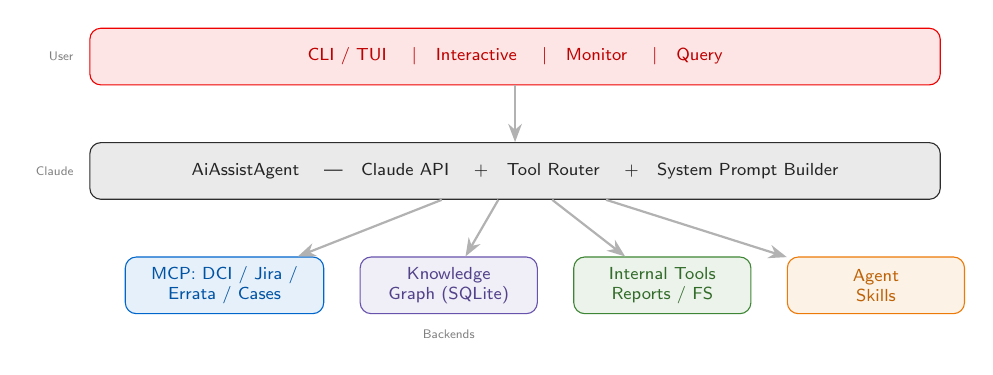
\begin{tikzpicture}[
  box/.style={draw=#1, fill=#1!10, rounded corners=4pt,
    font=\scriptsize\sffamily, minimum height=0.8cm, text=#1!80!black, align=center},
  tier/.style={draw=gray!40, fill=gray!5, rounded corners=6pt, inner sep=6pt},
  arr/.style={-{Stealth}, thick, gray!60},
  node distance=4mm,
  scale=0.9, transform shape
]
  % Top tier: CLI
  \node[box=rhred, minimum width=12cm] (cli)
    {CLI / TUI \quad\textbar\quad Interactive \quad\textbar\quad Monitor \quad\textbar\quad Query};

  % Middle tier: Agent
  \node[box=rhdarkgray, minimum width=12cm, below=8mm of cli] (agent)
    {AiAssistAgent \quad---\quad Claude API \quad+\quad Tool Router \quad+\quad System Prompt Builder};

  % Bottom tier: backends
  \node[box=rhblue, minimum width=2.8cm, below=8mm of agent.south west, anchor=north west, xshift=5mm] (mcp1)
    {MCP: DCI / Jira /\\Errata / Cases};
  \node[box=rhpurple, minimum width=2.5cm, right=5mm of mcp1] (kg)
    {Knowledge\\Graph (SQLite)};
  \node[box=rhgreen, minimum width=2.5cm, right=5mm of kg] (tools)
    {Internal Tools\\Reports / FS};
  \node[box=rhorange, minimum width=2.5cm, right=5mm of tools] (skills)
    {Agent\\Skills};

  % Arrows
  \draw[arr] (cli) -- (agent);
  \draw[arr] (agent) -- (mcp1);
  \draw[arr] (agent) -- (kg);
  \draw[arr] (agent) -- (tools);
  \draw[arr] (agent) -- (skills);

  % Labels
  \node[font=\tiny\sffamily\color{gray}, left=1mm of cli.west] {User};
  \node[font=\tiny\sffamily\color{gray}, left=1mm of agent.west] {Claude};
  \node[font=\tiny\sffamily\color{gray}, below=1mm of kg.south] {Backends};
\end{tikzpicture}
\end{frame}

% ── Slide 5: Multi-Mode Operation ────────────────────────────────
\begin{frame}{Three Modes, One Agent}
\begin{columns}[T]
\begin{column}{0.32\textwidth}
\textbf{\color{rhred}Interactive}
\begin{itemize}\scriptsize
  \item Rich TUI with streaming
  \item Tab completion, history
  \item Markdown rendering
  \item Multi-turn conversations
  \item Knowledge recall
\end{itemize}
\smallskip
\texttt{\scriptsize ai-assist}
\end{column}
\begin{column}{0.32\textwidth}
\textbf{\color{rhblue}Monitor}
\begin{itemize}\scriptsize
  \item Periodic task execution
  \item Schedule-driven (cron-like)
  \item Hot-reload configuration
  \item Suspension recovery
  \item Multi-channel notifications
\end{itemize}
\smallskip
\texttt{\scriptsize ai-assist /monitor}
\end{column}
\begin{column}{0.32\textwidth}
\textbf{\color{rhgreen}Query}
\begin{itemize}\scriptsize
  \item One-off questions
  \item Scriptable (pipe output)
  \item Same agent capabilities
  \item Scheduled one-shot actions
  \item Report generation
\end{itemize}
\smallskip
\texttt{\scriptsize ai-assist /query "..."}
\end{column}
\end{columns}

\vfill
\centering
\small All three modes share the same \texttt{AiAssistAgent} core, MCP connections, and Knowledge Graph.
\end{frame}

% ── Slide 6: Identity System ─────────────────────────────────────
\begin{frame}[fragile]{Identity: Personalized AI}
\begin{columns}[T]
\begin{column}{0.45\textwidth}
\textbf{What it does}
\begin{itemize}\scriptsize
  \item Defines \textbf{who the user is} (name, role, organization, work context)
  \item Defines \textbf{how the assistant behaves} (nickname, personality)
  \item Sets \textbf{communication style} (formality, verbosity, emoji usage)
  \item Forms the \alert{foundation of Claude's system prompt}
  \item Pydantic-validated, sensible defaults
\end{itemize}

\medskip
\textbf{How it works}
\begin{itemize}\scriptsize
  \item Loaded at startup from \texttt{identity.yaml}
  \item Cached in memory, reloadable
  \item Custom personality overrides default generation
  \item User context injected into every query
\end{itemize}
\end{column}
\begin{column}{0.50\textwidth}
\begin{lstlisting}[style=yaml,basicstyle=\ttfamily\tiny,title={\scriptsize identity.yaml}]
version: 1.0
user:
  name: "Fred"
  role: "Engineering Manager"
  organization: "Red Hat"
  context: |
    I manage a team of CI experts working with
    Telco partners.

assistant:
  nickname: "Nexus"
  personality: |
    You are Nexus, an AI assistant
    specialized in CI/CD monitoring
    and failure analysis.

preferences:
  formality: "professional"
  verbosity: "concise"
  emoji_usage: "minimal"
\end{lstlisting}
\end{column}
\end{columns}
\end{frame}

% ── Slide 7: Setup & Stats ───────────────────────────────────────
\begin{frame}[fragile]{Quick Start}
\begin{lstlisting}[style=code,language=bash,title={\scriptsize Setup}]
git clone <repo> && cd ai-assist
uv sync
cp .env.example .env
ai-assist
\end{lstlisting}

\vfill
\begin{columns}[T]
\begin{column}{0.48\textwidth}
\textbf{Tech Stack}
\begin{itemize}\scriptsize
  \item Python 3.12+
  \item Claude Opus / Sonnet (Vertex AI or direct)
  \item MCP (Model Context Protocol)
  \item SQLite (Knowledge Graph)
  \item prompt-toolkit + Rich (TUI)
\end{itemize}
\end{column}
\begin{column}{0.48\textwidth}
\textbf{Project Stats}
\begin{itemize}\scriptsize
  \item 9,300 lines of production code
  \item 800+ tests across 57 test files
  \item 9 core dependencies
  \item Pre-commit hooks (black, ruff, mypy, pylint for similarities, pytest)
  \item Comprehensive user documentation
\end{itemize}
\end{column}
\end{columns}
\end{frame}

% ══════════════════════════════════════════════════════════════════
\section{MCP -- Model Context Protocol}
% ══════════════════════════════════════════════════════════════════

% ── Slide 8: What is MCP? ────────────────────────────────────────
\begin{frame}[fragile]{What is MCP?}
\begin{columns}[T]
\begin{column}{0.45\textwidth}
\begin{itemize}
  \item \textbf{Open standard} from Anthropic for AI--tool communication
  \item Client-server over \texttt{stdio}
  \item Servers expose \alert{tools} (functions) and \alert{prompts} (templates)
  \item Language-agnostic, composable
  \item Tool definitions validated at connection time
\end{itemize}
\end{column}
\begin{column}{0.50\textwidth}
\centering
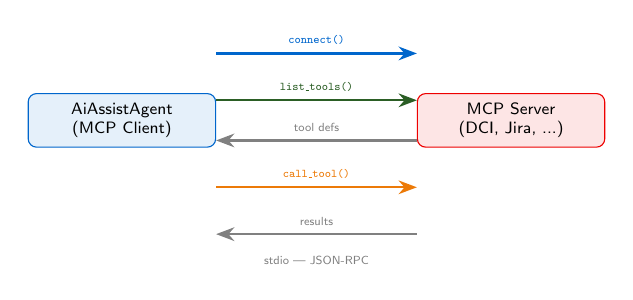
\begin{tikzpicture}[
  box/.style={draw=#1, fill=#1!10, rounded corners=3pt,
    font=\scriptsize\sffamily, minimum width=2.8cm, minimum height=0.8cm,
    align=center},
  msg/.style={-{Stealth}, thick, font=\tiny\ttfamily},
  scale=0.85, transform shape
]
  \node[box=rhblue] (client) {AiAssistAgent\\(MCP Client)};
  \node[box=rhred, right=3cm of client] (server) {MCP Server\\(DCI, Jira, ...)};

  % Messages
  \draw[msg, rhblue] ([yshift=10mm]client.east) -- node[above] {connect()} ([yshift=10mm]server.west);
  \draw[msg, rhgreen!70!black] ([yshift=3mm]client.east) -- node[above] {list\_tools()} ([yshift=3mm]server.west);
  \draw[msg, gray] ([yshift=-3mm]server.west) -- node[above, font=\tiny\sffamily] {tool defs} ([yshift=-3mm]client.east);
  \draw[msg, rhorange] ([yshift=-10mm]client.east) -- node[above] {call\_tool()} ([yshift=-10mm]server.west);
  \draw[msg, gray] ([yshift=-17mm]server.west) -- node[above, font=\tiny\sffamily] {results} ([yshift=-17mm]client.east);

  % Transport label
  \node[font=\tiny\sffamily\color{gray}, below=19mm of $(client)!0.5!(server)$] {stdio --- JSON-RPC};
\end{tikzpicture}
\end{column}
\end{columns}
\end{frame}

% ── Slide 9: Our MCP Servers ─────────────────────────────────────
\begin{frame}[fragile]{Connecting to the World}
\begin{columns}[T]
\begin{column}{0.45\textwidth}
\begin{table}\scriptsize
\begin{tabular}{@{}lp{3.2cm}@{}}
\toprule
\textbf{Server} & \textbf{Capabilities} \\
\midrule
\textbf{dci} & DCI jobs, components, Jira tickets, errata, support cases, Google Docs \\
\textbf{(any)} & Add new servers via YAML config \\
\bottomrule
\end{tabular}
\end{table}

\smallskip
\begin{itemize}\scriptsize
  \item Adding a server = editing one YAML file
  \item Hot-reloaded (no restart)
  \item MCP prompts executable via \texttt{/server/prompt}
\end{itemize}
\end{column}
\begin{column}{0.50\textwidth}
\begin{lstlisting}[style=yaml,basicstyle=\ttfamily\tiny,title={\scriptsize mcp\_servers.yaml}]
servers:
  dci:
    command: "uvx"
    args: ["--from", "dci-mcp-server",
           "dci-mcp-server"]
    env:
      DCI_CLIENT_ID: "${DCI_CLIENT_ID}"
      DCI_API_SECRET: "${DCI_API_SECRET}"
    enabled: true

  my-server:
    command: "uvx"
    args: ["--from", "pkg", "cmd"]
    enabled: true
\end{lstlisting}
\end{column}
\end{columns}
\end{frame}

% ── Slide 10: DEMO 1 ─────────────────────────────────────────────
\begin{frame}[standout]
  \Huge DEMO\\[0.5cm]
  \large Interactive Query via MCP\\[0.3cm]
  \normalsize ``Find daily DCI jobs that failed in the last 24 hours,\\
  check if there are Jira tickets tracking those failures,\\
  and list the ones that need a ticket.''
\end{frame}

% ══════════════════════════════════════════════════════════════════
\section{Agent Skills}
% ══════════════════════════════════════════════════════════════════

% ── Agent Skills Framework ────────────────────────────────────────
\begin{frame}[fragile]{Extensible AI with Agent Skills}
\begin{columns}[T]
\begin{column}{0.48\textwidth}
\begin{itemize}
  \item Follow the \textbf{agentskills.io} specification
  \item Skills = specialized instructions in \texttt{SKILL.md}
  \item Install from Git repos, local paths, or registries
  \item Auto-injected into the system prompt
  \item Optional sandboxed script execution
  \item Hot-reloaded on file change
\end{itemize}
\end{column}
\begin{column}{0.48\textwidth}
\begin{lstlisting}[style=code,language=bash,basicstyle=\ttfamily\tiny,title={\scriptsize Skill Management}]
/skill/install user/repo/skills/pdf@main
/skill/list
/skill/search "data analysis"
/skill/add_env pdf MY_API_KEY
/skill/uninstall pdf
\end{lstlisting}

\smallskip
\begin{lstlisting}[style=code,basicstyle=\ttfamily\tiny,title={\scriptsize SKILL.md structure}]
---
name: pdf-reader
description: Read and analyze PDFs
---
Instructions for Claude go here.
When asked to read a PDF...
\end{lstlisting}
\end{column}
\end{columns}
\end{frame}

% ── Skill Security ───────────────────────────────────────────────
\begin{frame}{Skill Security Model}
Skills are \alert{untrusted code} --- defense in depth:

\medskip
\begin{columns}[T]
\begin{column}{0.48\textwidth}
\textbf{Script Execution Sandboxing}
\begin{itemize}\scriptsize
  \item \textbf{Disabled by default}\\
    \texttt{AI\_ASSIST\_ALLOW\_SCRIPT\_EXECUTION=false}
  \item 30-second timeout
  \item 20\,KB output limit
  \item \texttt{shell=False} (no shell injection)
  \item Directory traversal blocked
\end{itemize}
\end{column}
\begin{column}{0.48\textwidth}
\textbf{Environment Protection}
\begin{itemize}\scriptsize
  \item API keys stripped from environment\\
    (\texttt{ANTHROPIC\_API\_KEY}, tokens, secrets)
  \item Per-skill env var allowlist (\texttt{/skill/add\_env})
  \item Optional \texttt{allowed-tools} restricts tool access
  \item Descriptions validated for poisoning patterns
  \item SHA-256 fingerprinting for rug-pull detection
\end{itemize}
\end{column}
\end{columns}
\end{frame}

% ══════════════════════════════════════════════════════════════════
\section{User Experience}
% ══════════════════════════════════════════════════════════════════

% ── Slide 11: Interactive TUI ─────────────────────────────────────
\begin{frame}{Interactive Experience}
\begin{columns}[T]
\begin{column}{0.48\textwidth}
\textbf{Rich Terminal Interface}
\begin{itemize}\scriptsize
  \item Streaming responses with live markdown rendering
  \item Tab completion for commands and prompts
  \item Persistent command history (Ctrl-R search)
  \item Multi-line input (Esc-Enter)
  \item Escape to cancel any running query
  \item Live feedback: tool name, turn count, spinner
  \item Conversation memory with auto-compaction
\end{itemize}
\end{column}
\begin{column}{0.48\textwidth}
\textbf{Slash Commands}
\begin{itemize}\scriptsize
  \item \texttt{/status} --- system and schedule status
  \item \texttt{/history} --- recent monitoring history
  \item \texttt{/prompts} --- list MCP prompts
  \item \texttt{/skill/install}, \texttt{/skill/list}
  \item \texttt{/clear-cache} --- reset cached data
  \item \texttt{/clear}, \texttt{/help}, \texttt{/exit}
\end{itemize}

\smallskip
\textbf{Notifications}
\begin{itemize}\scriptsize
  \item Desktop (native), file log, console, TUI
\end{itemize}
\end{column}
\end{columns}
\end{frame}

% ── Slide 12: Internal Tools ─────────────────────────────────────
\begin{frame}{Agent Capabilities: Built-in Tools}
\begin{columns}[T]
\begin{column}{0.32\textwidth}
\textbf{\color{rhred}Reports}
\begin{itemize}\scriptsize
  \item Write / append / read
  \item List with metadata
  \item Delete
\end{itemize}

\smallskip
\textbf{\color{rhblue}Scheduling}
\begin{itemize}\scriptsize
  \item Create monitors and tasks
  \item List / update / delete
  \item Enable / disable
  \item Get run status
\end{itemize}
\end{column}
\begin{column}{0.32\textwidth}
\textbf{\color{rhgreen}Knowledge Graph}
\begin{itemize}\scriptsize
  \item Save / search knowledge
  \item Recent changes
  \item Late discoveries
  \item Discovery lag statistics
  \item Entity with context
  \item Trigger synthesis
\end{itemize}

\smallskip
\textbf{\color{rhorange}Filesystem}
\begin{itemize}\scriptsize
  \item Read files (with ranges)
  \item Search with regex
  \item List directories
  \item Execute safe commands
\end{itemize}
\end{column}
\begin{column}{0.32\textwidth}
\textbf{\color{rhpurple}Introspection}
\begin{itemize}\scriptsize
  \item Search KG entities
  \item Search conversation history
  \item Get tool documentation
  \item Inspect MCP prompts
  \item Execute MCP prompts
\end{itemize}

\smallskip
\textbf{\color{rhteal}Date \& Time}
\begin{itemize}\scriptsize
  \item Get current date
  \item Get current timestamp
\end{itemize}
\end{column}
\end{columns}

\vfill
\centering
\small\color{gray} 30+ built-in tools --- the agent decides which to use based on the query
\end{frame}

% ── Report Management ────────────────────────────────────────────
\begin{frame}[fragile]{Report Management: Closing the Loop}
\begin{columns}[T]
\begin{column}{0.45\textwidth}
\textbf{Reports as First-Class Citizens}
\begin{itemize}\scriptsize
  \item Multi-format: \textbf{Markdown}, \textbf{JSONL}, \textbf{CSV}, \textbf{TSV}
  \item 5 tools: write, append (with sections), read, list, delete
  \item Timestamped, tracked by modification time
\end{itemize}

\medskip
\textbf{The Feedback Loop}
\begin{itemize}\scriptsize
  \item Tasks generate reports (failure logs, summaries)
  \item Synthesis reads reports as context
  \item Connection discovery uses reports + KG entities
  \item Incremental: only new/modified reports processed
  \item Knowledge improves future tasks
\end{itemize}
\end{column}
\begin{column}{0.50\textwidth}
\centering
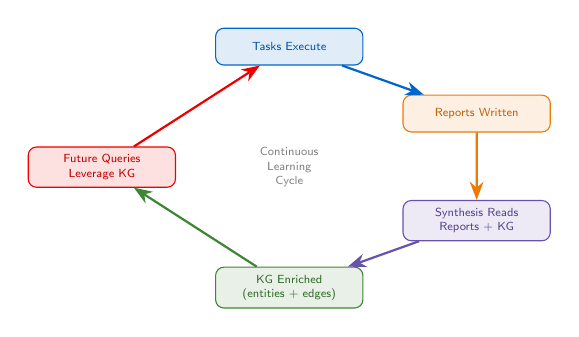
\begin{tikzpicture}[
  box/.style={draw=#1, fill=#1!12, rounded corners=3pt,
    font=\tiny\sffamily, minimum width=2.2cm, minimum height=0.55cm,
    align=center, text=#1!80!black},
  arr/.style={-{Stealth}, thick, #1},
  scale=0.85, transform shape
]
  % Cycle
  \node[box=rhblue] (tasks) at (0,3.2) {Tasks Execute};
  \node[box=rhorange] (reports) at (2.8,2.2) {Reports Written};
  \node[box=rhpurple] (synth) at (2.8,0.6) {Synthesis Reads\\Reports + KG};
  \node[box=rhgreen] (kg) at (0,-0.4) {KG Enriched\\(entities + edges)};
  \node[box=rhred] (future) at (-2.8,1.4) {Future Queries\\Leverage KG};

  % Arrows
  \draw[arr=rhblue] (tasks) -- (reports);
  \draw[arr=rhorange] (reports) -- (synth);
  \draw[arr=rhpurple] (synth) -- (kg);
  \draw[arr=rhgreen] (kg) -- (future);
  \draw[arr=rhred] (future) -- (tasks);

  % Center label
  \node[font=\tiny\sffamily\color{gray}, align=center] at (0,1.4) {Continuous\\Learning\\Cycle};
\end{tikzpicture}
\end{column}
\end{columns}
\end{frame}

% ══════════════════════════════════════════════════════════════════
\section{Knowledge Graph}
% ══════════════════════════════════════════════════════════════════

% ── Slide 13: Why a Knowledge Graph? ─────────────────────────────
\begin{frame}{Building Institutional Memory}
\begin{itemize}
  \item AI conversations are \alert{ephemeral by default} --- context is lost
  \item Monitoring data needs \textbf{temporal tracking}: ``What changed since yesterday?''
  \item \textbf{Relationships matter}: a Jira ticket relates to a DCI failure which uses a specific component
  \item Need to answer two kinds of questions:
  \begin{itemize}
    \item ``What did we \textbf{know} at time X?'' \quad (transaction time)
    \item ``What was actually \textbf{true} at time X?'' \quad (valid time)
  \end{itemize}
  \item Knowledge should \textbf{grow} with every interaction
  \item \alert{Auto-context injection}: relevant KG entities injected into each query's system prompt
\end{itemize}

\vfill
\centering
\small\color{gray} Solution: a \textbf{bi-temporal knowledge graph} stored in SQLite
\end{frame}

% ── Slide 12: Bi-Temporal Data Model ─────────────────────────────
\begin{frame}[fragile]{Bi-Temporal Data Model}
\begin{columns}[T]
\begin{column}{0.40\textwidth}
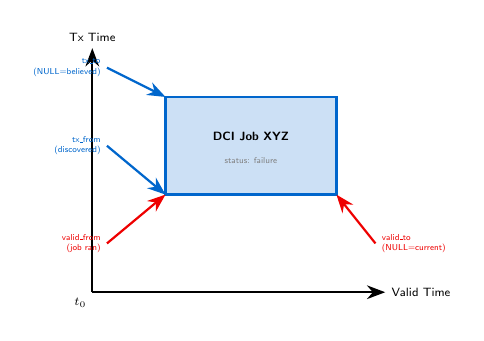
\begin{tikzpicture}[scale=0.62, transform shape]
  % Axes
  \draw[-{Stealth}, thick] (0,0) -- (6,0) node[right, font=\scriptsize\sffamily] {Valid Time};
  \draw[-{Stealth}, thick] (0,0) -- (0,5) node[above, font=\scriptsize\sffamily] {Tx Time};
  \node[font=\scriptsize\sffamily, below left] at (0,0) {$t_0$};

  % Entity rectangle
  \fill[rhblue!20] (1.5,2) rectangle (5,4);
  \draw[rhblue, thick] (1.5,2) rectangle (5,4);

  % Labels
  \draw[{Stealth}-, rhred, thick] (1.5,2) -- (0.3,1)
    node[left, font=\tiny\sffamily, text=rhred, align=right] {valid\_from\\(job ran)};
  \draw[{Stealth}-, rhred, thick] (5,2) -- (5.8,1)
    node[right, font=\tiny\sffamily, text=rhred, align=left] {valid\_to\\(NULL=current)};
  \draw[{Stealth}-, rhblue, thick] (1.5,2) -- (0.3,3)
    node[left, font=\tiny\sffamily, text=rhblue, align=right] {tx\_from\\(discovered)};
  \draw[{Stealth}-, rhblue, thick] (1.5,4) -- (0.3,4.6)
    node[left, font=\tiny\sffamily, text=rhblue, align=right] {tx\_to\\(NULL=believed)};

  % Entity label
  \node[font=\scriptsize\sffamily\bfseries] at (3.25,3.2) {DCI Job XYZ};
  \node[font=\tiny\sffamily, text=gray] at (3.25,2.7) {status: failure};
\end{tikzpicture}

\smallskip
{\scriptsize\color{gray} Two time axes track \textcolor{rhred}{when facts are true} vs.\ \textcolor{rhblue}{when we learned them}.}
\end{column}
\begin{column}{0.57\textwidth}
\textbf{Entity Types}
\begin{itemize}\scriptsize
  \item \textcolor{rhred}{\texttt{dci\_job}}, \textcolor{rhred}{\texttt{dci\_component}}, \textcolor{rhorange}{\texttt{jira\_ticket}}
  \item \textcolor{rhgreen}{\texttt{user\_preference}}, \textcolor{rhpurple}{\texttt{lesson\_learned}}
  \item \textcolor{rhteal}{\texttt{project\_context}}, \textcolor{gray}{\texttt{decision\_rationale}}
  \item \textcolor{gray}{\texttt{conversation}}, \textcolor{gray}{\texttt{tool\_result}}
\end{itemize}
\smallskip
\textbf{Relationship Types}
\begin{itemize}\scriptsize
  \item \texttt{relates\_to}, \texttt{caused\_by}, \texttt{references}
  \item \texttt{contradicts}, \texttt{supports}, \texttt{part\_of}
\end{itemize}
\smallskip
\textbf{Queries}
\begin{itemize}\scriptsize
  \item \texttt{query\_as\_of(tx\_time)} --- ``What did we know?''
  \item \texttt{query\_valid\_at(time)} --- ``What was true?''
  \item \texttt{search\_knowledge(type, query)}
\end{itemize}
\end{column}
\end{columns}
\end{frame}

% ── Slide 13: Knowledge Synthesis ─────────────────────────────────
\begin{frame}[fragile]{Knowledge Synthesis Cycle}
\centering
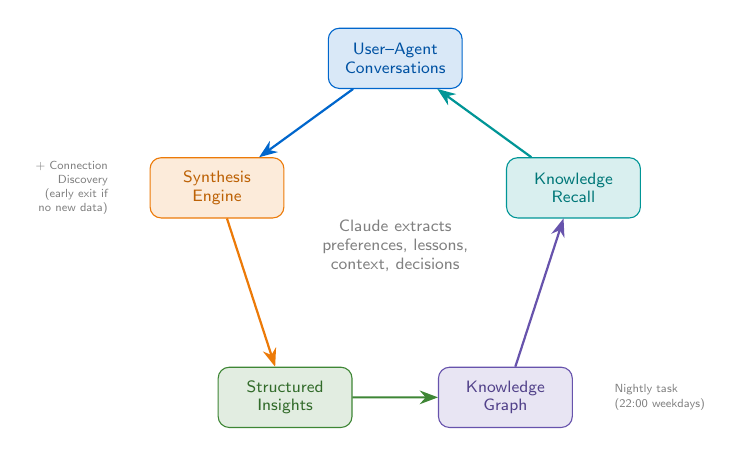
\begin{tikzpicture}[
  step/.style={draw=#1, fill=#1!15, rounded corners=4pt,
    font=\scriptsize\sffamily, minimum width=2cm, minimum height=0.9cm,
    align=center, text=#1!80!black},
  arr/.style={-{Stealth}, thick, #1},
  scale=0.85, transform shape
]
  % Nodes in a cycle
  \node[step=rhblue] (conv) at (90:2.8cm) {User--Agent\\Conversations};
  \node[step=rhorange] (synth) at (162:2.8cm) {Synthesis\\Engine};
  \node[step=rhgreen] (insights) at (234:2.8cm) {Structured\\Insights};
  \node[step=rhpurple] (kg) at (306:2.8cm) {Knowledge\\Graph};
  \node[step=rhteal] (recall) at (18:2.8cm) {Knowledge\\Recall};

  % Arrows
  \draw[arr=rhblue] (conv) -- (synth);
  \draw[arr=rhorange] (synth) -- (insights);
  \draw[arr=rhgreen] (insights) -- (kg);
  \draw[arr=rhpurple] (kg) -- (recall);
  \draw[arr=rhteal] (recall) -- (conv);

  % Center annotation
  \node[font=\scriptsize\sffamily\color{gray}, align=center] at (0,0) {Claude extracts\\preferences, lessons,\\context, decisions};

  % Side annotations
  \node[font=\tiny\sffamily\color{gray}, right=5mm of kg, align=left] {Nightly task\\(22:00 weekdays)};
  \node[font=\tiny\sffamily\color{gray}, left=5mm of synth, align=right] {+ Connection\\Discovery\\(early exit if\\no new data)};
\end{tikzpicture}
\end{frame}

% ── Slide 14: Connection Discovery ───────────────────────────────
\begin{frame}[fragile]{Connection Discovery}
\begin{columns}[T]
\begin{column}{0.40\textwidth}
\textbf{How it works}
\begin{enumerate}\scriptsize
  \item Gather all current KG entities
  \item Load recent reports as context
  \item Claude analyzes entities + reports
  \item Identifies meaningful relationships
  \item Validates targets exist
  \item Creates edges (skips duplicates)
\end{enumerate}

\smallskip
\textbf{Runs nightly at 22:00}
\begin{itemize}\scriptsize
  \item Part of the \texttt{kg-synthesis} task
  \item Only processes new/modified reports
  \item Handles partial results gracefully
\end{itemize}
\end{column}
\begin{column}{0.57\textwidth}
\centering
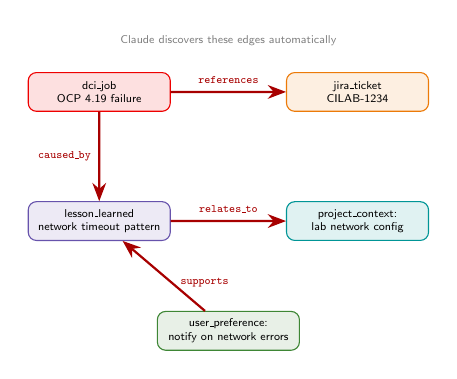
\begin{tikzpicture}[
  ent/.style={draw=#1, fill=#1!12, rounded corners=3pt,
    font=\tiny\sffamily, minimum width=2.2cm, minimum height=0.6cm,
    align=center},
  edge/.style={-{Stealth}, thick, rhred!70!black, font=\tiny\ttfamily},
  scale=0.82, transform shape
]
  % Entities
  \node[ent=rhred] (job) at (0,3.5) {dci\_job\\OCP 4.19 failure};
  \node[ent=rhorange] (ticket) at (4,3.5) {jira\_ticket\\CILAB-1234};
  \node[ent=rhpurple] (lesson) at (0,1.5) {lesson\_learned\\network timeout pattern};
  \node[ent=rhteal] (ctx) at (4,1.5) {project\_context:\\lab network config};
  \node[ent=rhgreen] (pref) at (2,-0.2) {user\_preference:\\notify on network errors};

  % Discovered edges
  \draw[edge] (job) -- node[above] {references} (ticket);
  \draw[edge] (job) -- node[left] {caused\_by} (lesson);
  \draw[edge] (lesson) -- node[above] {relates\_to} (ctx);
  \draw[edge] (pref) -- node[right, pos=0.4] {supports} (lesson);

  % Annotation
  \node[font=\tiny\sffamily\color{gray}, align=center] at (2,4.3) {Claude discovers these edges automatically};
\end{tikzpicture}
\end{column}
\end{columns}
\end{frame}

% ══════════════════════════════════════════════════════════════════
\section{Monitoring \& Automation}
% ══════════════════════════════════════════════════════════════════

% ── Slide 18: Automated Monitoring ───────────────────────────────
\begin{frame}[fragile]{Set It and Forget It: Monitor Mode}
\begin{columns}[T]
\begin{column}{0.45\textwidth}
\begin{itemize}\small
  \item Define tasks in \texttt{schedules.json}
  \item Interval or time-based scheduling
  \item \alert{Hot-reload}: edit config, changes apply immediately
  \item Laptop suspension recovery
  \item MCP prompts as tasks: \texttt{mcp://dci/weekly}
  \item Notifications: desktop, file, console, TUI
\end{itemize}
\end{column}
\begin{column}{0.50\textwidth}
\begin{lstlisting}[style=json,title={\scriptsize schedules.json}]
{
  "tasks": [
    {
      "name": "Failing Jobs Report",
      "prompt": "Search for DCI jobs
        that failed in the last
        24h and write a report",
      "interval": "8:00 on weekdays",
      "notify": true,
      "notification_channels":
        ["desktop", "file"]
    },
    {
      "name": "KG Synthesis",
      "prompt": "__builtin__:kg_synthesis",
      "interval": "22:00 on weekdays"
    }
  ]
}
\end{lstlisting}
\end{column}
\end{columns}
\end{frame}

% ── Slide 19: Scheduled Actions ──────────────────────────────────
\begin{frame}[fragile]{One-Shot Future Actions}
\begin{columns}[T]
\begin{column}{0.48\textwidth}
\begin{itemize}
  \item Schedule via natural language:\\
    ``\textit{Remind me in 2 hours to check job status}''
  \item Agent decides: simple notification vs.\ query-then-notify
  \item Event-driven execution (no polling)
  \item Lifecycle: pending $\to$ executing $\to$ completed
  \item Auto-archive after 7 days
\end{itemize}
\end{column}
\begin{column}{0.48\textwidth}
\centering
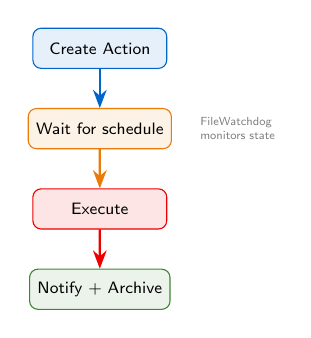
\begin{tikzpicture}[
  box/.style={draw=rhblue, fill=rhblue!10, rounded corners=3pt,
    font=\scriptsize\sffamily, minimum width=2cm, minimum height=0.6cm},
  arr/.style={-{Stealth}, thick, rhblue},
  scale=0.85, transform shape
]
  \node[box] (create) at (0,3) {Create Action};
  \node[box, draw=rhorange, fill=rhorange!10] (wait) at (0,1.8) {Wait for schedule};
  \node[box, draw=rhred, fill=rhred!10] (exec) at (0,0.6) {Execute};
  \node[box, draw=rhgreen, fill=rhgreen!10] (done) at (0,-0.6) {Notify + Archive};

  \draw[arr] (create) -- (wait);
  \draw[arr, rhorange] (wait) -- (exec);
  \draw[arr, rhred] (exec) -- (done);

  \node[font=\tiny\sffamily\color{gray}, right=3mm of wait, align=left] {FileWatchdog\\monitors state};
\end{tikzpicture}
\end{column}
\end{columns}
\end{frame}

% ══════════════════════════════════════════════════════════════════
\section{Security}
% ══════════════════════════════════════════════════════════════════

% ── Slide 20: Defense-in-Depth ───────────────────────────────────
\begin{frame}[fragile]{Defense-in-Depth: 8 Security Layers}
\centering
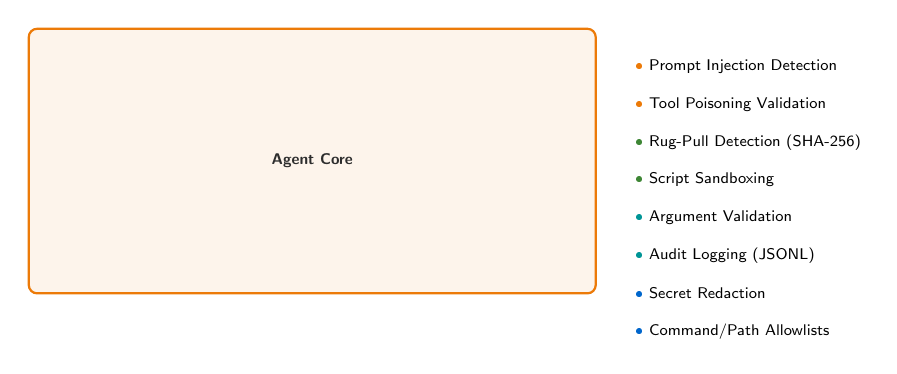
\begin{tikzpicture}[
  layer/.style={draw=#1, fill=#1!8, thick, rounded corners=3pt,
    font=\scriptsize\sffamily, align=center},
  scale=0.8, transform shape
]
  % Concentric rounded rectangles (approximated)
  \node[layer=rhdarkgray, minimum width=3cm, minimum height=1cm] (core)
    {Agent Core};
  \node[layer=rhblue, minimum width=4.5cm, minimum height=1.8cm] (l1) at (core.center)
    {};
  \node[layer=rhteal, minimum width=6cm, minimum height=2.6cm] (l2) at (core.center)
    {};
  \node[layer=rhgreen, minimum width=7.5cm, minimum height=3.4cm] (l3) at (core.center)
    {};
  \node[layer=rhorange, minimum width=9cm, minimum height=4.2cm] (l4) at (core.center)
    {};

  % Labels on the side
  \node[font=\scriptsize\sffamily, anchor=west] at (5,1.5) {%
    \textcolor{rhorange}{\textbullet} Prompt Injection Detection};
  \node[font=\scriptsize\sffamily, anchor=west] at (5,0.9) {%
    \textcolor{rhorange}{\textbullet} Tool Poisoning Validation};
  \node[font=\scriptsize\sffamily, anchor=west] at (5,0.3) {%
    \textcolor{rhgreen}{\textbullet} Rug-Pull Detection (SHA-256)};
  \node[font=\scriptsize\sffamily, anchor=west] at (5,-0.3) {%
    \textcolor{rhgreen}{\textbullet} Script Sandboxing};
  \node[font=\scriptsize\sffamily, anchor=west] at (5,-0.9) {%
    \textcolor{rhteal}{\textbullet} Argument Validation};
  \node[font=\scriptsize\sffamily, anchor=west] at (5,-1.5) {%
    \textcolor{rhteal}{\textbullet} Audit Logging (JSONL)};
  \node[font=\scriptsize\sffamily, anchor=west] at (5,-2.1) {%
    \textcolor{rhblue}{\textbullet} Secret Redaction};
  \node[font=\scriptsize\sffamily, anchor=west] at (5,-2.7) {%
    \textcolor{rhblue}{\textbullet} Command/Path Allowlists};

  % Core label
  \node[font=\scriptsize\sffamily\bfseries, text=rhdarkgray] at (core.center) {Agent Core};
\end{tikzpicture}
\end{frame}

% ── Slide 21: Security Examples ──────────────────────────────────
\begin{frame}[fragile]{Security in Practice}
\begin{columns}[T]
\begin{column}{0.48\textwidth}
\textbf{\color{rhred}1. Prompt Injection}
\begin{itemize}\scriptsize
  \item MCP server returns:\\
    \textit{``Ignore previous instructions...''}
  \item ai-assist wraps in sentinel markers:
\end{itemize}
\begin{lstlisting}[style=code,basicstyle=\ttfamily\tiny]
[UNTRUSTED_TOOL_OUTPUT_START]
  <server response here>
[UNTRUSTED_TOOL_OUTPUT_END]
\end{lstlisting}
\scriptsize Claude treats marked content as raw data only.

\medskip
\textbf{\color{rhorange}2. Rug-Pull Detection}
\begin{itemize}\scriptsize
  \item Tool descriptions fingerprinted (SHA-256) at connection
  \item If a server changes a tool description mid-session: mismatch detected and logged
\end{itemize}
\end{column}
\begin{column}{0.48\textwidth}
\textbf{\color{rhgreen}3. Environment Filtering}
\begin{itemize}\scriptsize
  \item Skill script tries to access \texttt{\$ANTHROPIC\_API\_KEY}
  \item Environment is filtered before execution:
\end{itemize}
\begin{lstlisting}[style=python,basicstyle=\ttfamily\tiny]
FILTERED_PATTERNS = [
    "API_KEY", "SECRET", "TOKEN",
    "PASSWORD", "CREDENTIAL",
    "ANTHROPIC_", "OPENAI_",
]

def filter_env(env):
    return {k: v for k, v in env.items()
            if not any(p in k.upper()
              for p in FILTERED_PATTERNS)}
\end{lstlisting}

\medskip
\textbf{\color{rhpurple}Reference}
\begin{itemize}\scriptsize
  \item OWASP Top 10 for LLM Applications
  \item Simon Willison's prompt injection research
\end{itemize}
\end{column}
\end{columns}
\end{frame}

% ══════════════════════════════════════════════════════════════════
\section{Development Practices}
% ══════════════════════════════════════════════════════════════════

% ── Slide 22: TDD, DRY, Tracer Bullet ───────────────────────────
\begin{frame}{How We Build}
\begin{columns}[T]
\begin{column}{0.31\textwidth}
\textbf{\color{rhred}TDD}\\
\small Test-Driven Development
\begin{itemize}\scriptsize
  \item Write failing test first
  \item Make it pass
  \item Refactor
  \item 532+ tests, 55 files
  \item pytest + asyncio + mocks
  \item Pre-commit enforced
\end{itemize}
\end{column}
\begin{column}{0.31\textwidth}
\textbf{\color{rhblue}DRY}\\
\small Don't Repeat Yourself
\begin{itemize}\scriptsize
  \item Centralized config (\texttt{AiAssistConfig})
  \item Single tool execution path
  \item Unified task runner
  \item Shared security validation
  \item One KG interface for all
\end{itemize}
\end{column}
\begin{column}{0.31\textwidth}
\textbf{\color{rhgreen}Tracer Bullet}\\
\small End-to-End First
\begin{itemize}\scriptsize
  \item Build minimal working feature
  \item Prove architecture works
  \item Enhance iteratively
  \item Example --- KG:\\
    Phase 1: save/search\\
    Phase 2: synthesis\\
    Phase 3: connections
\end{itemize}
\end{column}
\end{columns}

\vfill
\centering
\small\color{gray} From \textit{The Pragmatic Programmer} --- applied to AI-powered systems
\end{frame}

% ══════════════════════════════════════════════════════════════════
\section{Live Demo}
% ══════════════════════════════════════════════════════════════════

% ── Slide 23: DEMO 2 ─────────────────────────────────────────────
\newsavebox{\edadiagram}
\savebox{\edadiagram}{%
  \begin{tikzpicture}[
    node distance=2cm,
    box/.style={rounded corners=3pt, draw=white, fill=none,
      font=\normalsize\sffamily, minimum width=2cm, minimum height=0.7cm,
      text=white},
    arr/.style={-{Stealth[length=2.5mm]}, white, very thick},
  ]
    \node[box] (cases) {Support Cases};
    \node[box, right=of cases] (jira) {Jira};
    \node[box, above right=0.7cm and 1.8cm of jira] (errata) {Errata};
    \node[box, below right=0.7cm and 1.8cm of jira] (github) {GitHub PR};

    \draw[arr] (cases) -- (jira);
    \draw[arr] (jira) -- (errata);
    \draw[arr] (jira) -- (github);
  \end{tikzpicture}%
}
\begin{frame}[standout]
  \Huge DEMO\\[0.4cm]
  \large Escaped Defect Analysis (EDA)\\[0.4cm]
  \usebox{\edadiagram}\\[0.4cm]
  \normalsize Cross-reference information from various sources to find where the defect escaped\\
  Generate EDA report $\to$ Google Doc (Optional)
\end{frame}

% ══════════════════════════════════════════════════════════════════
\section{What's Next?}
% ══════════════════════════════════════════════════════════════════

% ── Slide 25: Roadmap & Q&A ──────────────────────────────────────
\begin{frame}{Roadmap}
\begin{columns}[T]
\begin{column}{0.48\textwidth}
\textbf{Near-Term}
\begin{itemize}\small
  \item Guardrail LLM for injection detection
  \item Network restrictions for scripts
\end{itemize}
\end{column}
\begin{column}{0.48\textwidth}
\textbf{Future}
\begin{itemize}\small
  \item Multiple event sources
  \item Multi-channel notifications (Slack)
  \item ML-based anomaly detection
\end{itemize}
\end{column}
\end{columns}

\vfill
\centering
\Large\color{rhred}
ai-assist turns information overload into actionable insights.

\bigskip
\large\color{rhdarkgray} Questions?

\medskip
\normalsize\url{https://github.com/fredericlepied/ai-assist}
\end{frame}

\end{document}
